% Chapter Template

\chapter{Ensayos y resultados} % Main chapter title

\label{Chapter4} % Change X to a consecutive number; for referencing this chapter elsewhere, use \ref{ChapterX}

%----------------------------------------------------------------------------------------
%	CHAPTER 4
%----------------------------------------------------------------------------------------

En este capítulo se explica cómo se llevaron a cabo las pruebas de validación de hardware y software a las que fue sometido el dispositivo, los bancos de ensayos, instrumentos utilizados y los resultados obtenidos.

\section{Instrumental utilizado}

Para poder ejecutar las pruebas de integración de hardware y software se requirió del uso de una variedad de instrumentos y componentes en los bancos de ensayos. La tabla \ref{tab:instrumentos} lista los detalles de cada uno de ellos.

\begin{table}[H]
	\centering
	\caption{Lista de instrumental utilizado.}
	\begin{tabular}{p{3cm} c p{6cm}}
		\toprule
		\textbf{Item} & \textbf{Modelo} & \textbf{Descripción} \\
		\midrule
		Multímetro			& UNI-T UT61A		& Multímetro digital autorango de alta precisión. \\
		Fuente de tensión	& KM GP-300ATX		& Fuente de computadora de 400 W. \\
		Resistencia de potencia variable		& AVT05006E25R00KE	& Resistencia de potencia de alambre bobinado de 25 Ohm / 50 W. \\
		Potenciómetro							& 3590S-1-201L & Potenciómetro de 200 Ohm / 2 W y 10 vueltas para panel. \\
		Conversor USB a UART					& EM7-6043		& Conversor USB a serie TTL CH-340. \\
		Cables varios							& - 			& Cables dupont y unipolar de 2,5 mm2. \\
		PC										& -				& Computadora de escritorio con software PuTTY (cliente de terminal). \\
		\bottomrule
		\hline
	\end{tabular}
	\label{tab:instrumentos}
\end{table}

\section{Banco de ensayos}

En la figura \ref{tab:instrumentos} se puede ver una foto de 

%\ref{fig:setupEnsayos}

%\begin{figure}[H]
%\centering
%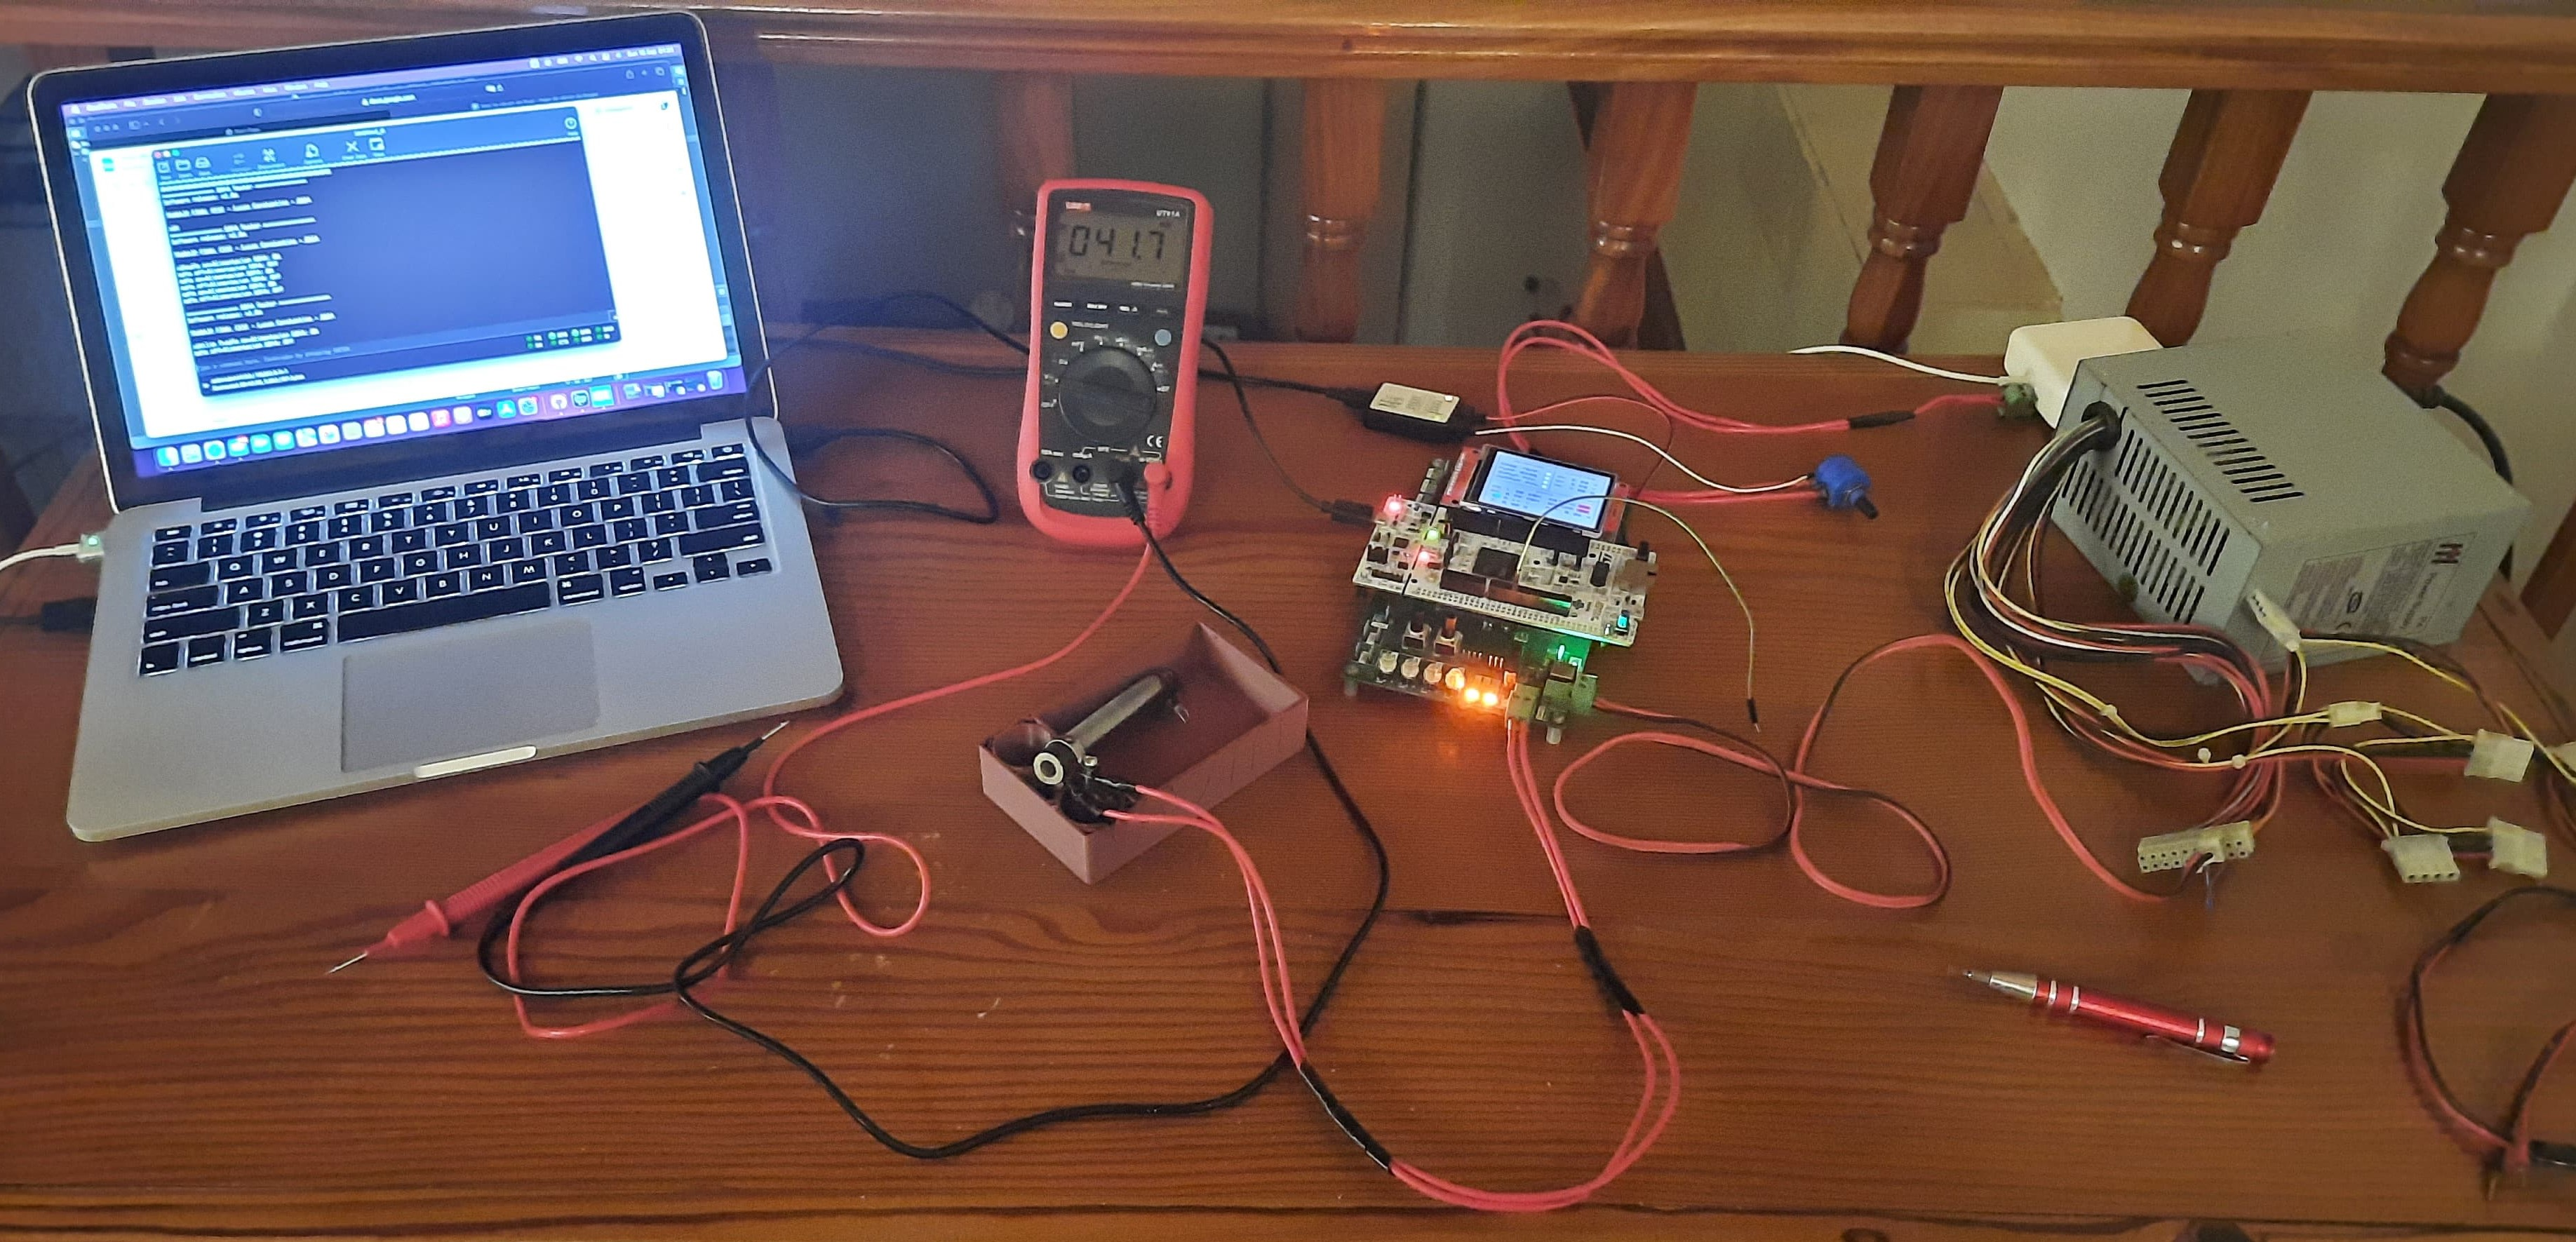
\includegraphics[width=0.75\textwidth]{./Figures/setupEnsayos.png}
%\caption{Esquema del monitor de corriente}
%\label{fig:setupEnsayos}
%\end{figure}

\section{Pruebas de hardware}
\label{sec:pruebasHW}

% mencionar aca que hay algunas pruebas de hardware como la del monitor de tension y de las señales analogicas que no tiene sentido probarlas porque son triviales

en este caso, el diseño del dispositivo no es complejo y el funcionamiento de las distintas partes del hardware es trivial. En general, solo basta con medir continuidad o valores de tensión en ciertos puntos para concluir que funcionan correctamente. Los únicos casos para los cuales es necesario realizar una prueba

\subsection{Pruebas del monitor de corriente}



\subsection{Pruebas del relé de alimentación}



\section{Pruebas de firmware}
\label{sec:pruebasFW}



\subsection{Pruebas del monitor de tensión}



\subsection{Pruebas del monitor de corriente}



\subsection{Pruebas de la pantalla LCD}

\subsection{Pruebas de la pantalla táctil}

\subsection{Pruebas de la comunicación UART}

\subsection{Pruebas de las alarmas y señales de control}
% mostrar directamente que se prenden en la pantalla tactil ???

\section{Pruebas de integración}
\label{sec:pruebasInt}

Las pruebas de integración tienen como objetivo probar la interacción del hardware y el firmware entre sí, es decir, el funcionamiento del sistema como una unidad.